\documentclass[border=8pt]{standalone}
\usepackage[T1]{fontenc}\usepackage[utf8]{inputenc}
\usepackage{helvet}\renewcommand{\familydefault}{\sfdefault}
\usepackage{tikz,xcolor}
\usetikzlibrary{arrows.meta,positioning,shapes.geometric,shapes.multipart,calc,fit,backgrounds,decorations.markings}
\definecolor{ink}{HTML}{1E1B16}\definecolor{paper}{HTML}{FBF8F2}\definecolor{clay}{HTML}{B5482A}\definecolor{soft}{HTML}{F1E9DA}\definecolor{pine}{HTML}{24402F}
\tikzset{
  every node/.style={font=\small,text=ink},
  >=Stealth, line/.style={draw=ink,line width=0.8pt},
  cls/.style={rectangle split,rectangle split parts=3,draw=ink,line width=0.8pt,fill=soft,align=left,inner xsep=6pt,inner ysep=4pt,
              rectangle split part align={center,left,left},minimum width=3.0cm},
  cls2/.style={rectangle split,rectangle split parts=2,draw=ink,line width=0.8pt,fill=soft,align=left,inner xsep=6pt,inner ysep=4pt,
              rectangle split part align={center,left},minimum width=3.0cm},
  box/.style={rectangle,draw=ink,line width=0.8pt,fill=soft,align=center,inner sep=5pt,minimum height=0.8cm},
  state/.style={rectangle,rounded corners=8pt,draw=ink,line width=0.8pt,fill=soft,align=center,inner sep=6pt,minimum width=2.2cm,minimum height=0.9cm},
  act/.style={rectangle,rounded corners=10pt,draw=ink,line width=0.8pt,fill=soft,align=center,inner sep=5pt,minimum width=2.4cm,minimum height=0.8cm},
  dec/.style={diamond,draw=ink,line width=0.8pt,fill=soft,inner sep=1pt,minimum width=0.9cm,minimum height=0.9cm},
  uc/.style={ellipse,draw=ink,line width=0.8pt,fill=soft,align=center,inner sep=3pt,minimum width=3.2cm,minimum height=1.0cm},
  note/.style={rectangle,draw=ink,line width=0.6pt,fill=yellow!12,align=left,inner sep=4pt,font=\footnotesize},
  lab/.style={font=\footnotesize,fill=paper,inner sep=1.5pt},
  err/.style={},
}
\newcommand{\actor}[3]{% x,y,label
  \draw[line width=0.8pt] (#1,#2+0.55) circle (0.17);
  \draw[line width=0.8pt] (#1,#2+0.38)--(#1,#2-0.15) (#1-0.3,#2+0.22)--(#1+0.3,#2+0.22) (#1,#2-0.15)--(#1-0.25,#2-0.6) (#1,#2-0.15)--(#1+0.25,#2-0.6);
  \node[font=\small] at (#1,#2-0.9) {#3};}
\begin{document}
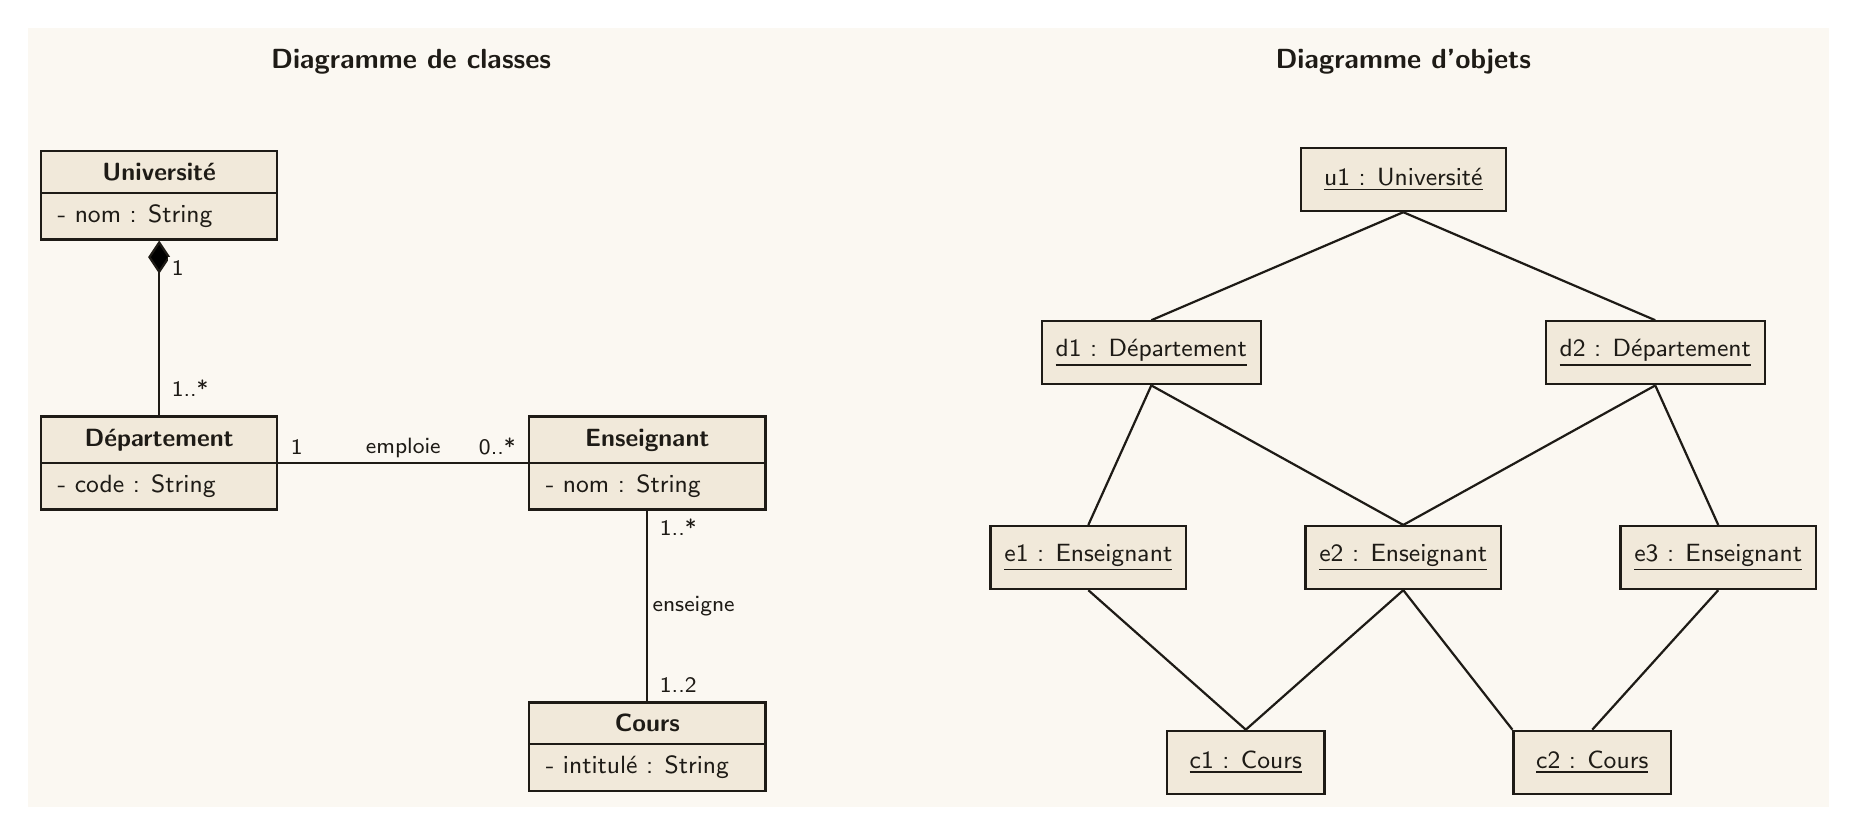
\begin{tikzpicture}[background rectangle/.style={fill=paper},show background rectangle]
\node[font=\bfseries] at (3.6,6.3) {Diagramme de classes};
\node[cls2,minimum width=3.0cm] (U) at (0.4,4.6) {\textbf{Université}\nodepart{two}- nom : String};
\node[cls2,minimum width=3.0cm] (D) at (0.4,1.2) {\textbf{Département}\nodepart{two}- code : String};
\node[cls2,minimum width=3.0cm] (E) at (6.6,1.2) {\textbf{Enseignant}\nodepart{two}- nom : String};
\node[cls2,minimum width=3.0cm] (C) at (6.6,-2.4) {\textbf{Cours}\nodepart{two}- intitulé : String};
\draw[line,{Diamond[length=12pt,width=8pt]}-] (U.south)--(D.north);
\node[lab,anchor=west] at ([xshift=0.1cm,yshift=-0.35cm]U.south) {1};
\node[lab,anchor=west] at ([xshift=0.1cm,yshift=0.35cm]D.north) {1..*};
\draw[line,] (D.east)--(E.west) node[midway,above,lab]{emploie};
\node[lab,anchor=south west] at ([xshift=0.1cm,yshift=0.05cm]D.east) {1};
\node[lab,anchor=south east] at ([xshift=-0.1cm,yshift=0.05cm]E.west) {0..*};
\draw[line,] (E.south)--(C.north) node[midway,right,lab]{enseigne};
\node[lab,anchor=north west] at ([xshift=0.1cm,yshift=-0.05cm]E.south) {1..*};
\node[lab,anchor=south west] at ([xshift=0.1cm,yshift=0.05cm]C.north) {1..2};
\node[font=\bfseries] at (16.2,6.3) {Diagramme d'objets};
\node[box,minimum width=2.6cm] (u1) at (16.2,4.8) {\underline{u1 : Université}};
\node[box,minimum width=2.4cm] (d1) at (13.0,2.6) {\underline{d1 : Département}};
\node[box,minimum width=2.4cm] (d2) at (19.4,2.6) {\underline{d2 : Département}};
\node[box,minimum width=2.2cm] (e1) at (12.2,0.0) {\underline{e1 : Enseignant}};
\node[box,minimum width=2.2cm] (e2) at (16.2,0.0) {\underline{e2 : Enseignant}};
\node[box,minimum width=2.2cm] (e3) at (20.2,0.0) {\underline{e3 : Enseignant}};
\node[box,minimum width=2.0cm] (c1) at (14.2,-2.6) {\underline{c1 : Cours}};
\node[box,minimum width=2.0cm] (c2) at (18.6,-2.6) {\underline{c2 : Cours}};
\draw[line] (u1.south)--(d1.north);
\draw[line] (u1.south)--(d2.north);
\draw[line] (d1.south)--(e1.north);
\draw[line] (d1.south)--(e2.north);
\draw[line] (d2.south)--(e3.north);
\draw[line] (e1.south)--(c1.north);
\draw[line] (e2.south)--(c1.north);
\draw[line] (e2.south)--(c2.north west);
\draw[line] (e3.south)--(c2.north);
\draw[line] (d2.south)--(e2.north);
\end{tikzpicture}
\end{document}
